\chapter{Experiments} \label{experiments}
In this chapter, we present results of three experiments which we carried out
in order to estimate the performance of our system and to explore different
hyperparameter settings. The outcomes of these experiments can determine the
direction of future research on our system and enable us to compare
it with reference data.

The first two experiments were aimed at discovering relations between
particular hyperparameter settings. In the first experiment
(section \ref{sec:exp:sample}) we compare the two
sampling strategies which were presented in section \ref{sec:scoresample}.
The second experiment focuses on genetic operators; we tried to determine
whether the result changes if we turn one of these operators off
(section \ref{sec:exp:genop}). 

The goal of the last experiment was to evaluate our system on benchmark
datasets and compare the results with reference data
(section \ref{sec:exp:openml}). We used the OpenML-CC18 benchmarking suite for
this purpose \citep{openmlcc18}.

\section{Sampling strategies} \label{sec:exp:sample}
In section \ref{sec:scoresample} we presented two different performance
estimation strategies aimed at reducing the evaluation time. Both methods
are based on sampling of the full dataset, but the generation of the samples
differs --- either a sample of the original dataset is generated for every
individual evaluation (\emph{per-ind}), or only once per generation
(\emph{per-gen}), and it is shared by all individuals. The goal of this experiment
was to test whether one approach is better and, if possible, to compare it with
evaluation on the complete dataset (the \emph{full} strategy).

The strategies were tested on three different datasets:

\begin{itemize}
\item wilt --- Medium size dataset (4839 instances, 6 features), the task is to
detect diseased trees in image segments. There are two target classes: `w' (diseased
trees) and `n' (all other land cover). The dataset is heavily unbalanced; only
261 instances of the `w' class are present
\citep{doi:10.1080/01431161.2013.810825}.
\item wine-quality-white --- Medium size dataset (4898 instances, 12 features),
the features represent properties of a particular Portuguese wine. Each of the
wines has been graded by three experts according to sensory properties, the
target value is a median of these grades. The task is to predict the target
grading (1--7), which may be either a classification or a regression task.
We solve it as a classification task \citep{CORTEZ2009547}.
\item MagicTelescope (magic) --- Large dataset (19020 instances, 12 features)
the task is to determine whether the data produced by the Cherenkov gamma
telescope describes a `signal' or only `background data' \citep{BOCK2004511}.
\end{itemize}

\paragraph{Setting}

% TODO weights?
\begin{table}[ht]

\centering
\caption{System hyperparameters for the sampling experiment}\label{tab04:exp1:setting}
\begin{tabular}{l c}
\toprule
\textbf{\upshape Hyperparameter} & \textbf{Value} \\
\midrule
population size & 200 \\
maximum generation & 15 \\
crossover probability & 0.5 \\
subtree mutation probability & 0.3 \\
node argument mutation probability & 0.6 \\
node mutation probability & 0.3 \\
maximum tree height & 5 \\
timeout per method  & 7 minutes \\
group weights & \textit{default} \\
\bottomrule

\end{tabular}

\end{table}

The sample size was chosen proportionally to the dataset size to sufficiently
reduce the running time --- $\frac{1}{4}$ of all instances in case of the
medium-sized datasets and $\frac{1}{20}$ for the magic dataset. During the
evolution, the individual fitness was computed as 5-fold cross-validation on
the samples, or on the full dataset respectively. The final evaluation method of
resulting optimized pipelines was 10 times 10-fold cross-validation on
the full dataset.

Hyperparameter settings of the system are presented in Table
\ref{tab04:exp1:setting}, their influence on the system is discussed in Chapter
\ref{our:solution}.
For the wilt dataset we used Cohen's kappa
as the scoring method \citep{doi:10.1177/001316446002000104}. Cohen's kappa is a statistic used to measure agreement
of the classifier with the `ground truth', with values ranging from -1.0 to 1.0.
Value of -1.0 corresponds to complete disagreement, 1.0 to complete agreement
and 0.0 is equivalent to random guessing. The reason why this more specific
statistic was used is that due to wilt being an unbalanced dataset, the
cross-validation accuracy score is close to 1.0 and differences between
run results may not be apparent. With Cohen's kappa having a wider range of values,
the differences can be observed in more detail.

\paragraph{Results}

% Stats exp 1
\begin{table}[ht]
\centering
\caption{Boxplot statistics of the sample experiment (magic)}\label{tab04:exp1:magboxstats}

\begin{tabular}{lrrrr|c}
\toprule
{} &  minimum &  median &  confidence interval &  maximum & eval.\,time\textsuperscript{1} \\
\midrule
per\_gen &   0.8645 &  0.8792 & $(0.8773,0.8811)$ &    0.882 & 28 min \\
per\_ind &   0.8720 &  0.8795 & $(0.8772,0.8819)$ &    0.882 & 34 min \\
\bottomrule

\multicolumn{6}{l}{\footnotesize\textsuperscript{1}\itshape Evaluation time of the first generation}

\end{tabular}

\end{table}

\begin{table}[ht]
\centering
\caption{Boxplot statistics of the sample experiment (wilt)}\label{tab04:exp1:wboxstats}

\begin{tabular}{lrrrr|c}
\toprule
{} &  minimum & median & confidence interval &  maximum & eval.\,time\textsuperscript{1} \\
\midrule
full     &   0.8695 &  0.8798 &   $(0.8736,0.8861)$ &   0.8908 & 25 min \\
per\_gen &   0.8684 &  0.8730 &   $(0.8699,0.8760)$ &   0.8878 & 11 min \\
per\_ind &   0.8661 &  0.8736 &   $(0.8708,0.8764)$ &   0.8877 & 6 min \\
\bottomrule

\multicolumn{6}{l}{\footnotesize\textsuperscript{1}\itshape Evaluation time of the first generation}

\end{tabular}

\end{table}

\begin{table}[ht]
\centering
\caption{Boxplot statistics of the sample experiment (wine-quality-white)}\label{tab04:exp1:wineboxstats}

\begin{tabular}{lrrrr|c}
\toprule
{} &  minimum &  median & confidence interval &  maximum & eval.\,time\textsuperscript{1} \\
\midrule
full     &   0.5524 &  0.7059 &   $(0.6491,0.7627)$ &   0.7097 & 53 min \\
per\_gen &   0.5295 &  0.5391 &   $(0.5372,0.5409)$ &   0.5518 & 27 min \\
per\_ind &   0.5340 &  0.5380 &   $(0.5343,0.5417)$ &   0.5454 & 35 min \\
\bottomrule

\multicolumn{6}{l}{\footnotesize\textsuperscript{1}\itshape Evaluation time of the first generation}

\end{tabular}

\end{table}

% Boxplots exp 1
\begin{figure}[b!]\centering
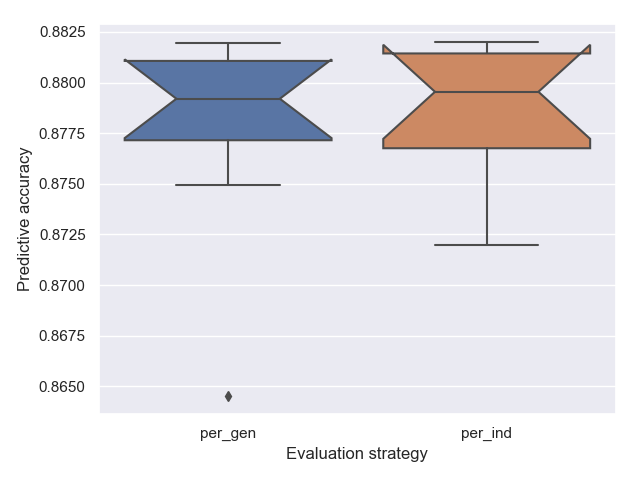
\includegraphics[width=0.8\textwidth]{../img/magic-out.png}
\caption{Comparison of strategies on the magic dataset}
\label{pic04:magic}
\end{figure}

\begin{figure}[pt]\centering
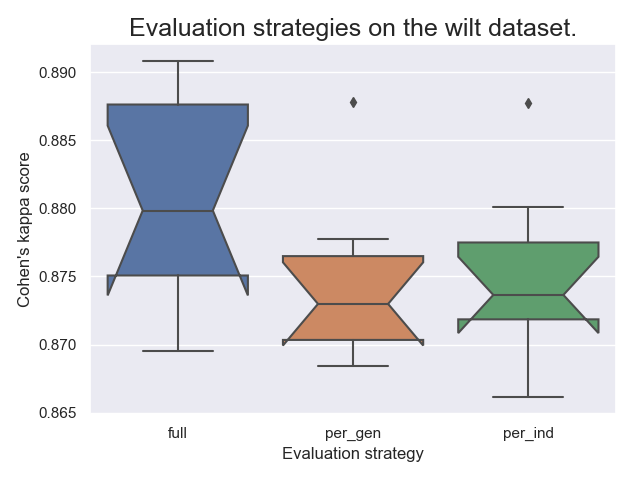
\includegraphics[width=0.8\textwidth]{../img/wilt-out.png}
\caption{Comparison of strategies on the wilt dataset}
\label{pic04:wilt}
\end{figure}

\begin{figure}[pt]\centering
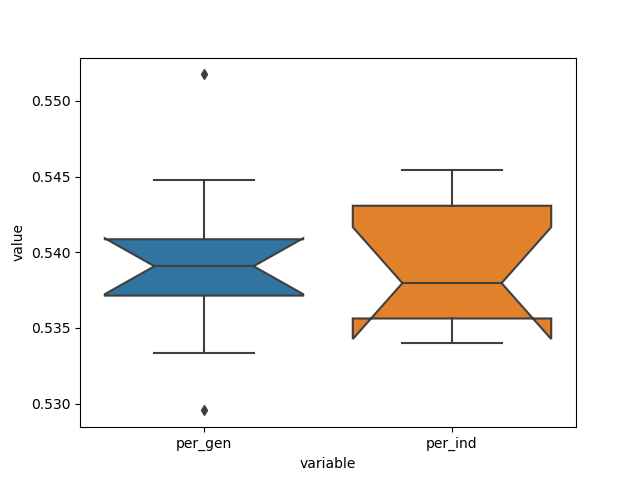
\includegraphics[width=0.8\textwidth]{../img/winequality-out.png}
\caption{Comparison of strategies on the wine-quality-white dataset}
\label{pic04:winequality}
\end{figure}

For each run we have chosen 5 pipelines with the highest score
from the Pareto front, or the full Pareto front if it had been shorter than 5
pipelines. These pipelines were again evaluated using the 10-fold
cross-validation. Finally, the maximum of the scores was chosen. Figures
\ref{pic04:magic}, \ref{pic04:wilt} and \ref{pic04:winequality} visualize the
distribution of the 10 scores per strategy. Relevant statistics of the
boxplots are listed in Tables \ref{tab04:exp1:magboxstats},
\ref{tab04:exp1:wboxstats}, \ref{tab04:exp1:wineboxstats}.
We also list the evaluation times of the first generation in the tables. As the
evaluation time greatly depends on generated pipelines, the differences in running
times are subject to random fluctuations and are listed only for illustration.


In the figures, middle line of the boxplot represents the median, while notches determine the
95\% confidence interval of the median. The whiskers determine the minimum and
maximum values respectively (without outliers). The lower and upper edges of
the box represent the first and the third quartile respectively.
% TODO whiskers, quartiles redundant, maybe? Reader knows boxplot definition? 

In all of the experiments we found no statistically significant difference
between per-gen and per-ind methods. However, not counting
the outliers, per-ind method had a greater variance in all three cases.

The full strategy has been shown to be significantly better on the
wine-quality-white dataset. On the wilt dataset, although most of the scores
resulting from the full method were better than results of the methods
using sampling, the 95\% confidence intervals of all strategies overlap. As
such, it is not possible to say that the full method is significantly
better than the sampling. In addition to that, its result scores had a great
variance in both cases.

The overall conclusion from this experiment is that on small datasets, or when the
longer duration is not overly limiting, the full
method should be preferred. In other cases the per-gen method with a reasonable
sample size is a good compromise.


\section{Combinations of genetic operators} \label{sec:exp:genop}
The goal of this experiment was to test whether the absence of some genetic
operators influences the result score. The motivation is that if we observe a
significant difference in results, we can focus on improving a particular
genetic operator or alter the default probability settings.

We used two datasets with different properties:
\begin{itemize}
\item wilt --- Medium sized dataset, see section \ref{sec:exp:sample}
\item climate-model-simulation-crashes (climate) --- Small dataset (540
instances, 21 features), the task is to predict whether a particular
climate model simulation crashes due to numerical or other reasons
\citep{gmd-6-1157-2013}.
\end{itemize}

\paragraph{Setting}

As described in section \ref{sec:repro}, there is one crossover operator and
three mutation operators --- the point mutation (or node mutation), subtree
mutation and hyperparameter
mutation. The following sub-experiments were performed:
\begin{itemize}
\setlength\itemsep{0.3em}
\item \textbf{all} --- all genetic operators included
\item \textbf{no-arg} --- hyperparameter mutation turned off
\item \textbf{no-cx} --- crossover turned off
\item \textbf{no-node} --- node mutation turned off
\item \textbf{no-subtree} --- subtree crossover turned off
\item \textbf{nothing} -- all genetic operators turned off
\end{itemize}
In every sub-experiment all operators that are not excluded keep their default
probabilities. The probabilities and other system hyperparameter
settings are listed in Table \ref{tab04:exp2:setting}, with a more detailed
explanation of their meaning in Chapter \ref{our:solution}.
Sample size for the wilt dataset was the same as in section
\ref{sec:exp:sample}, the evaluation strategy was per-gen. We did not use any
sampling with the climate dataset, as it has only a small number of samples and features.
For fitness computation we used the 5-fold cross-validation. Final evaluation
and data collection was the same as in the previous experiment --- for each run we
have chosen 5 pipelines with the highest score from the Pareto front
(or less, if the Pareto front was smaller). These pipelines were once again
evaluated using the 10-fold cross-validation. The maximum of the scores was chosen
as the overall result of the run.

\begin{table}[ht]
\centering
\caption{System hyperparameters for the genetic operator experiment}\label{tab04:exp2:setting}
\begin{tabular}{l c}
\toprule
\textbf{\upshape Hyperparameter} & \textbf{Value} \\
\midrule
population size & 200 \\
maximum generation & 15 \\
crossover probability & 0.5 \\
subtree mutation probability & 0.3 \\
node argument mutation probability & 0.6 \\
node mutation probability & 0.3 \\
maximum tree height & 5 \\
timeout per method  & 7 minutes \\
group weights & \textit{default} \\
\bottomrule

\end{tabular}

\end{table}

\paragraph{Results}
The results of this experiment are depicted in Figures \ref{pic04:mut-wilt} and
\ref{pic04:mut-climate}, with boxplot statistics listed in Tables
\ref{tab04:exp2:wboxstats} and \ref{tab04:exp2:cboxstats}. Again, the evaluation
time of the first generation is listed only for illustration purpose.

In case of the wilt dataset, only the `no-arg' method did not introduce any improvement
when compared to results from the setting with no genetic operators (`nothing').
This probably means that the
hyperparameter mutation is essential on this dataset --- in fact, the best
pipelines usually contained a SVC, which relies heavily on hyperparameter
optimization \citep{Feurer:2015:ERA:2969442.2969547}.

The `no-node' configuration was significantly better than almost all other methods
on the climate dataset (some of the confidence interval slightly overlap though).
The reason of this is not apparent and this behaviour may be one of the subjects
of future research.

The confidence intervals of medians of the `nothing' method and of the other methods,
except for the `no-node' setting on climate dataset, overlap. A possible explanation may be that
there still is a chance that a good individual is found during the
initialization, thus producing a better final score. The conclusion is that the
genetic operators and corresponding probabilities need to be tuned to reliably
produce better pipelines than those generated in the first generation.

\begin{table}[ht]
\centering
\caption{Boxplot statistics of the genetic operators experiment (wilt)}\label{tab04:exp2:wboxstats}
\begin{tabular}{lrrrr|c}
\toprule
{} &  minimum &  median &  confidence interval &  maximum & eval.\,time\textsuperscript{1} \\
\midrule
all        &   0.8658 &  0.8749 &   $(0.8711,0.8786)$ &   0.8820 & 9 min \\
no-arg     &   0.8526 &  0.8694 &   $(0.8684,0.8703)$ &   0.8794 & 7 min \\
no-cx      &   0.8499 &  0.8748 &   $(0.8715,0.8781)$ &   0.8875 & 10 min \\
no-node    &   0.8664 &  0.8747 &   $(0.8721,0.8772)$ &   0.8864 & 10 min \\
no-subtree &   0.8675 &  0.8738 &   $(0.8706,0.8770)$ &   0.8850 & 4 min \\
nothing    &   0.8434 &  0.8659 &   $(0.8585,0.8734)$ &   0.8787 & 3 min \\
\bottomrule

\multicolumn{6}{l}{\footnotesize\textsuperscript{1}\itshape Evaluation time of the first generation}

\end{tabular}

\end{table}

\begin{table}[ht]
\centering
\caption{Boxplot statistics of the genetic operators experiment (climate)}\label{tab04:exp2:cboxstats}
\begin{tabular}{lrrrr|c}
\toprule
{} &  minimum & median &  confidence interval &  maximum  & eval.\,time\textsuperscript{1} \\
\midrule
all        &   0.9112 &  0.9167 &   $(0.9135, 0.9200)$ &   0.9280 & 2 min \\
no-arg     &   0.9149 &  0.9159 &   $(0.9140, 0.9177)$ &   0.9296 & 9 min \\
no-cx      &   0.9111 &  0.9168 &   $(0.9152, 0.9184)$ &   0.9242 & 8 min \\
no-node    &   0.9149 &  0.9223 &   $(0.9199, 0.9247)$ &   0.9259 & 8 min \\
no-subtree &   0.9112 &  0.9177 &   $(0.9155, 0.9200)$ &   0.9316 & 5 min \\
nothing    &   0.9055 &  0.9149 &   $(0.9133, 0.9165)$ &   0.9185 & 2 min \\
\bottomrule

\multicolumn{6}{l}{\footnotesize\textsuperscript{1}\itshape Evaluation time of the first generation}

\end{tabular}

\end{table}

\begin{figure}[pt]\centering
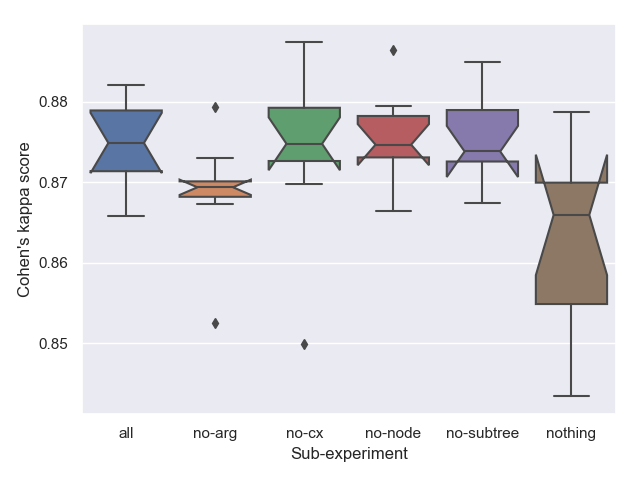
\includegraphics[width=0.8\textwidth]{../img/wilt-mut-redo.png}
\caption{Test of genetic operators on the wilt dataset}
\label{pic04:mut-wilt}
\end{figure}

\begin{figure}[pt]\centering
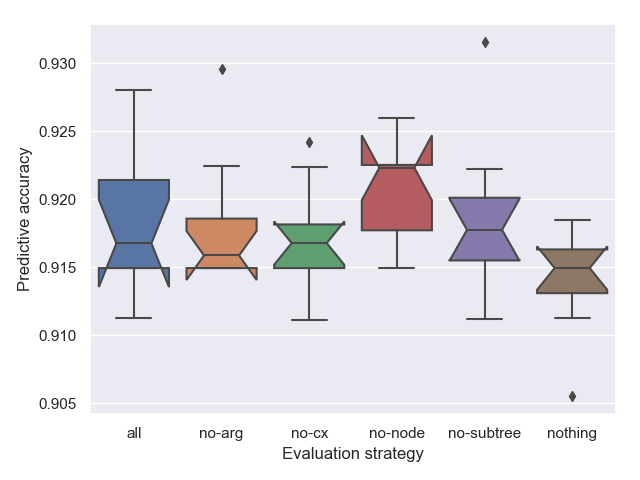
\includegraphics[width=0.8\textwidth]{../img/climate-mut-redo.png}
\caption{Test of genetic operators on the climate dataset}
\label{pic04:mut-climate}
\end{figure}

\section{OpenML-CC18 benchmarking suite} \label{sec:exp:openml}
% OpenML-CC18
% benchmark description

OpenML is a machine learning environment designed for sharing of machine
learning problem data \citep{OpenML2013}. It provides a variety of datasets
along with tasks and metadata of past runs. The data is accessible via APIs
available for several programming languages, notably Python or R
\citep{openmlcc18docs}. OpenML classifies the components of solving a
machine learning problem into following categories:
\begin{itemize}
\item Datasets --- The datasets are stored along with description and other
metadata.
\item Tasks --- A task is associated with a particular dataset. An example of a
task is 10 times 10-fold cross-validation on the dataset.
\item Flows --- A flow describes a specific machine learning algorithm.
\item Runs --- A run is a record of a flow with specified hyperparameters
applied to a task.
\end{itemize}
There are also several concept in development, like a study, which is a
collection of data from above-mentioned categories.

In this experiment we have used a study named OpenML-CC18 \citep{openmlcc18}.
This collection is a set of classification tasks created for the purpose
of practical benchmarking. It contains 72 datasets which have been frequently
used in recently published benchmarks and also satisfy several criteria, like
a limit on instance count or reasonable task difficulty. The full list of
criteria can be found in the OpenML documentation \citep{openmlcc18docs}.
Every dataset is associated with one task --- a 10-fold cross-validation. 
Majority of the tasks has already a great number of runs recorded along it,
therefore the suite can be used as reference data for our runs.

\paragraph{Setting}
In order to reduce the overall running time, sample size has been chosen
according to dataset size, as can be seen in Table \ref{tab04:exp3:size}.
If the product of feature count and instance count was less than $10,000$,
no sampling was performed.
The sizes were chosen in a heuristic manner by examining duration of runs
from section \ref{sec:exp:sample} and \ref{sec:exp:genop}.

Table \ref{tab04:exp3:setting} lists hyperparameter settings (their purpose
is described in Chapter \ref{our:solution}) for all of the
benchmark runs. Although we showed in section \ref{sec:exp:sample}
that the per-ind method had a greater variance, it was used here as this
experiment preceded the sample experiment. For fitness computation, we used
5-fold cross-validation on a sample. The final evaluation was the 10-fold
cross-validation on the full dataset as specified by the task definition.

\begin{table}[ht]

\centering
\caption{Sample size in relation to the dataset size (OpenML-CC18 experiment)}\label{tab04:exp3:size}
\begin{tabular}{l D{.}{.}{1.2}}
\toprule
\textbf{Row count limit} & \textbf{Sample size} \\
\midrule
small, less than $10,000$ entries\textsuperscript{1} & 1.0 \\
$1,000$ & 0.5 \\
$5,000$ & 0.25 \\
$10,000$ & 0.1 \\
$20,000$ & 0.05 \\
large, less than 10 features & 0.02 \\
large, more than 10 features & 0.01 \\
\bottomrule

\multicolumn{2}{l}{\footnotesize
\textsuperscript{1}\textit{Datasets of small number of features and
instances were not sampled}} \\

\end{tabular}

\end{table}

\begin{table}[ht]

\centering
\caption{System hyperparameters for the OpenML-CC18 experiment}\label{tab04:exp3:setting}
\begin{tabular}{l c}
\toprule
\textbf{\upshape Hyperparameter} & \textbf{Value} \\
\midrule
population size & 200 \\
maximum generation & 15 \\
crossover probability & 0.5 \\
subtree mutation probability & 0.3 \\
node argument mutation probability & 0.6 \\
node mutation probability & 0.3 \\
maximum tree height & 5 \\
timeout per method  & 7 minutes \\
evaluation strategy & per-ind \\
evaluation metric & predictive accuracy \\
group weights & \textit{default} \\
\bottomrule

\end{tabular}

\end{table}

\paragraph{Results}
Figures \ref{fig:OpenML:boxplot:0}, \ref{fig:OpenML:boxplot:1},
\ref{fig:OpenML:boxplot:2} and \ref{fig:OpenML:boxplot:3} show the results
of our runs compared with results of runs uploaded to OpenML. For every dataset
we have done only one run due to time limitations. For each run we have
evaluated top 3 pipelines from the Pareto front and selected the maximum score.
Data from runs uploaded to OpenML were extracted using the OpenML python API
\citep{openmlcc18api}.

The boxplots represent the distribution of predictive accuracies from all runs
on a particular dataset, while the red circle marks the score of our run.
It should be noted that the number of runs varies
greatly between different datasets; some datasets are associated with more
than $100,000$ runs, while others only with hundreds of runs or even less. Thus,
the appearance of some boxplots may be skewed. Full statistics can be found on
the OpenML web page or using the OpenML API \citep{openmlcc18, openmlcc18docs}.

As can be seen from the plots, on most of the benchmark datasets our systems
found a pipeline which scored above the upper quartile or only slightly below
it. In some cases the score was equal or very close to the overall maximum. On
the \emph{madelon} dataset we found a pipeline which performed better than the
maximum run score recorded in OpenML.

The datasets which were problematic for our system were notably the
\emph{jungle\_chess} \footnote{Full dataset name, as in OpenML:
\emph{jungle\_chess\_2pcs\_raw\_endgame\_complete}} dataset, 
and \emph{CIFAR-10}. The jungle\_chess dataset is associated with only
about $3,700$ runs on only few flows. Most of the flow pipelines contained a
SVC, which performed particularly well on this dataset. Thus, our system did
not find the optimal SVC hyperparameter configuration (or a better pipeline),
but we cannot determine the relation to other yet to be tested flows.

In case of the CIFAR-10 dataset, there were only 76 runs. Moreover, most of the
runs were from flows representing keras models \citep{chollet2015keras}. These
are deep neural networks with a very large hyperparameter configuration space
and several layers, which is beyond the scope of our system as we use only
machine learning methods from scikit-learn.

Our system also performed less well on some small datasets. Usually, a more
complex model was one of the individuals with the biggest fitness, but the
resulting score was lower than the score of some simpler models. This may have
happened due to overfitting, and should be solved in following versions of our
system by employing a more elaborate evaluation method.

% TODO maybe violin plot?

\begin{sidewaysfigure}[ht]
    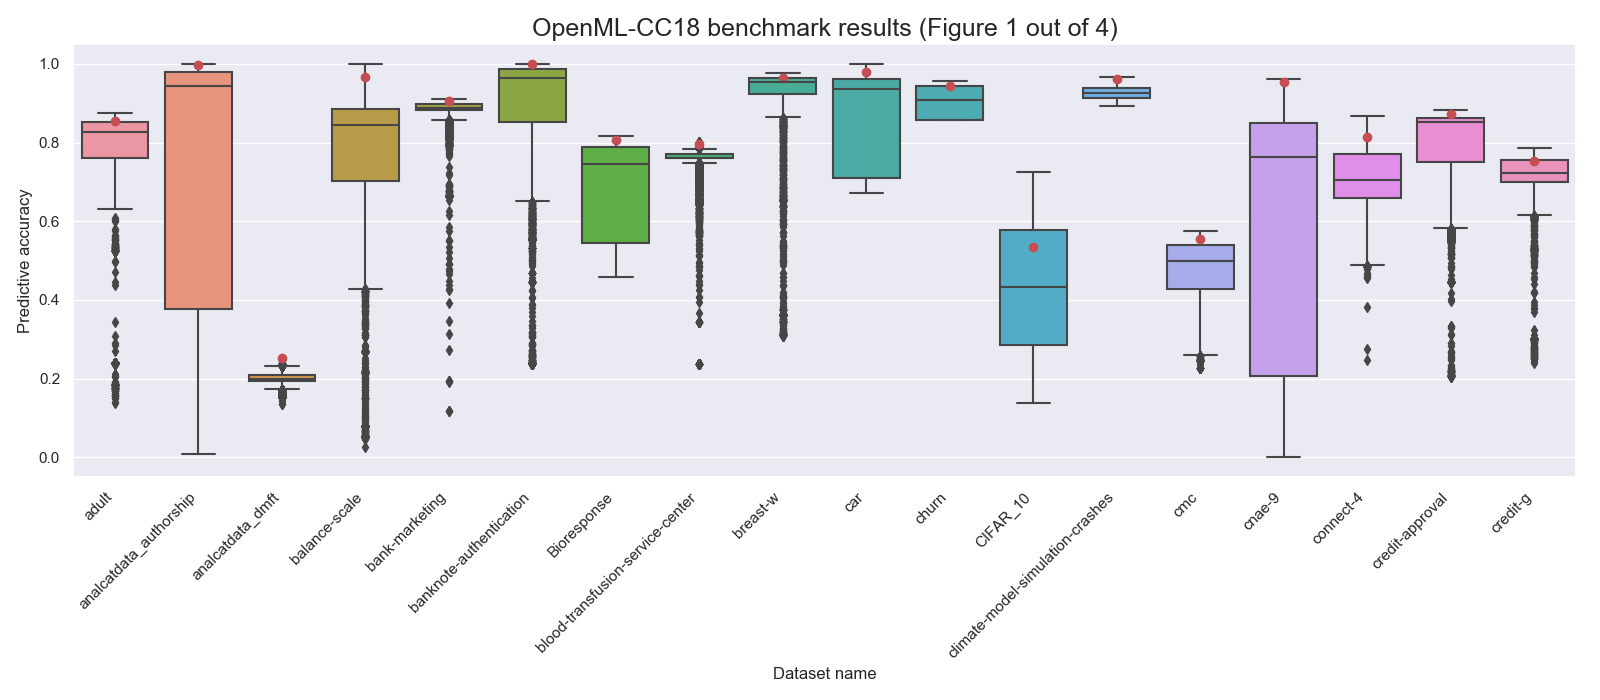
\includegraphics[width=\textwidth]{../img/openml-boxplot0.png}
    \caption[OpenML-CC18 benchmark result compad rison (Figure 1 out of 4)]{
    OpenML-CC18 benchmark result comparison (Figure 1 out of 4).
    Boxplots visualize distributions of predictive accuracies of all
    runs uploaded to OpenML. Red circles mark our accuracy score on datasets.}
    \label{fig:OpenML:boxplot:0}
\end{sidewaysfigure}

\begin{sidewaysfigure}[ht]
    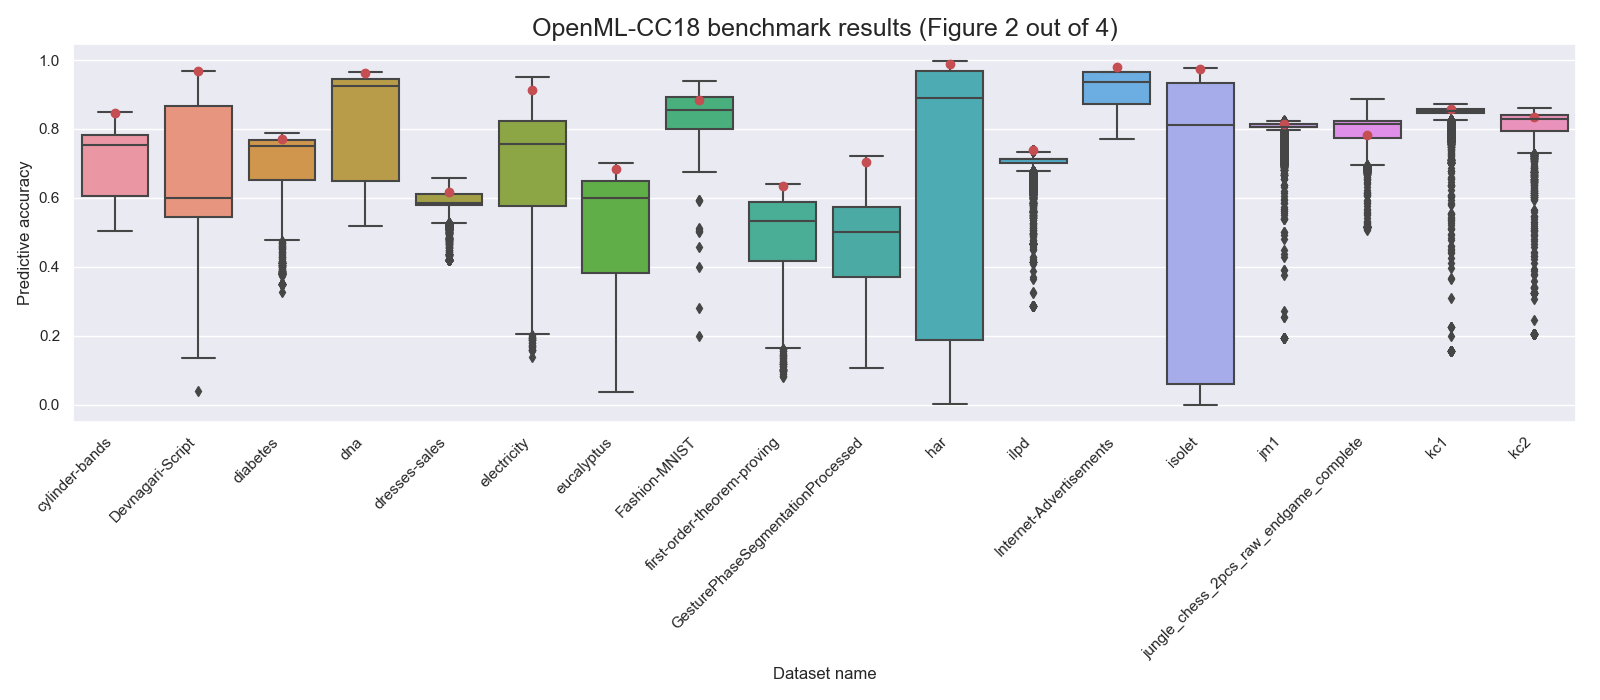
\includegraphics[width=\textwidth]{../img/openml-boxplot1.png}
    \caption[OpenML-CC18 benchmark result comparison (Figure 2 out of 4)]{
	OpenML-CC18 benchmark result comparison (Figure 2 out of 4).    
    Boxplots visualize distributions of predictive accuracies of all
    runs uploaded to OpenML. Red circles mark our accuracy score on datasets.}
    \label{fig:OpenML:boxplot:1}
\end{sidewaysfigure}

\begin{sidewaysfigure}[ht]
    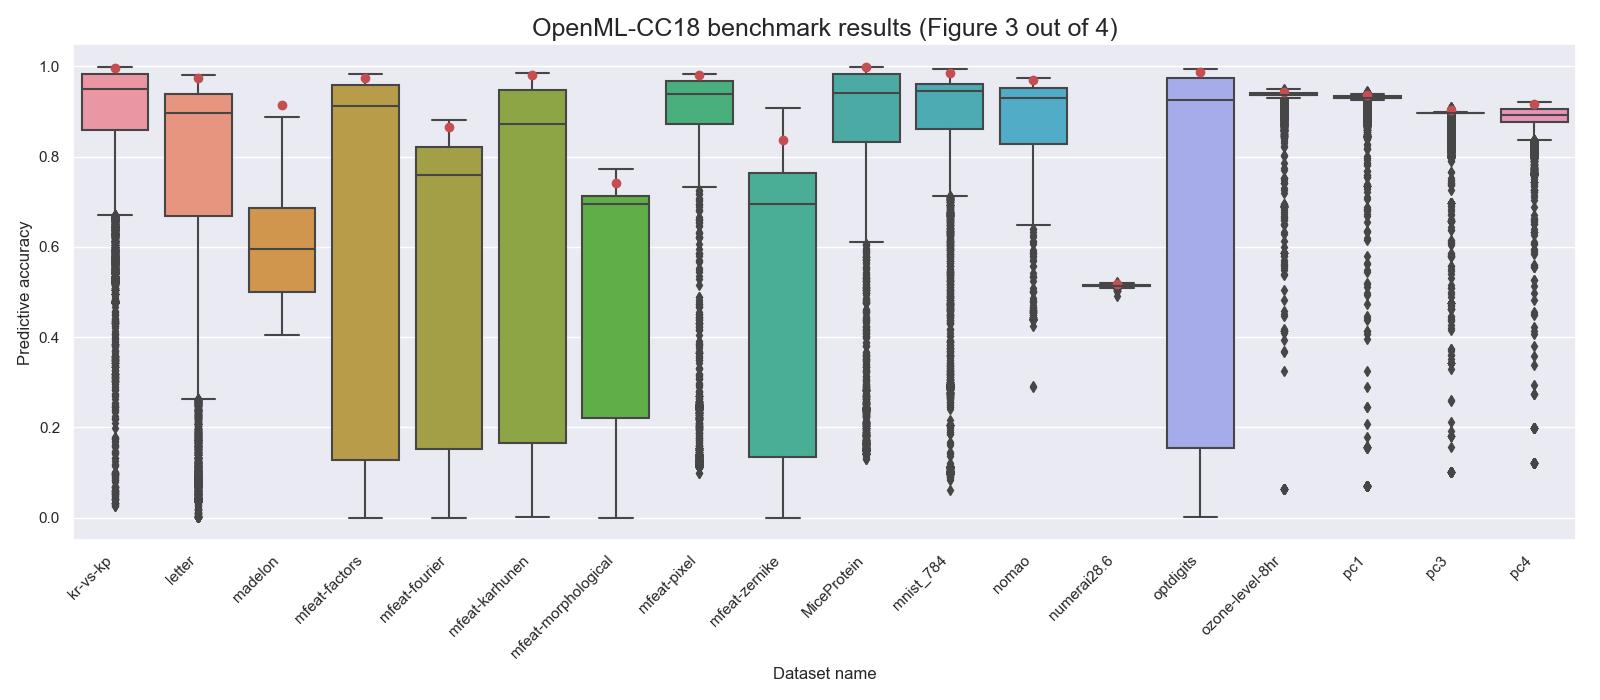
\includegraphics[width=\textwidth]{../img/openml-boxplot2.png}
    \caption[OpenML-CC18 benchmark result comparison (Figure 3 out of 4)]{
	OpenML-CC18 benchmark result comparison (Figure 3 out of 4).    
    Boxplots visualize distributions of predictive accuracies of all
    runs uploaded to OpenML. Red circles mark our accuracy score on datasets.}
    \label{fig:OpenML:boxplot:2}
\end{sidewaysfigure}

\begin{sidewaysfigure}[ht]
    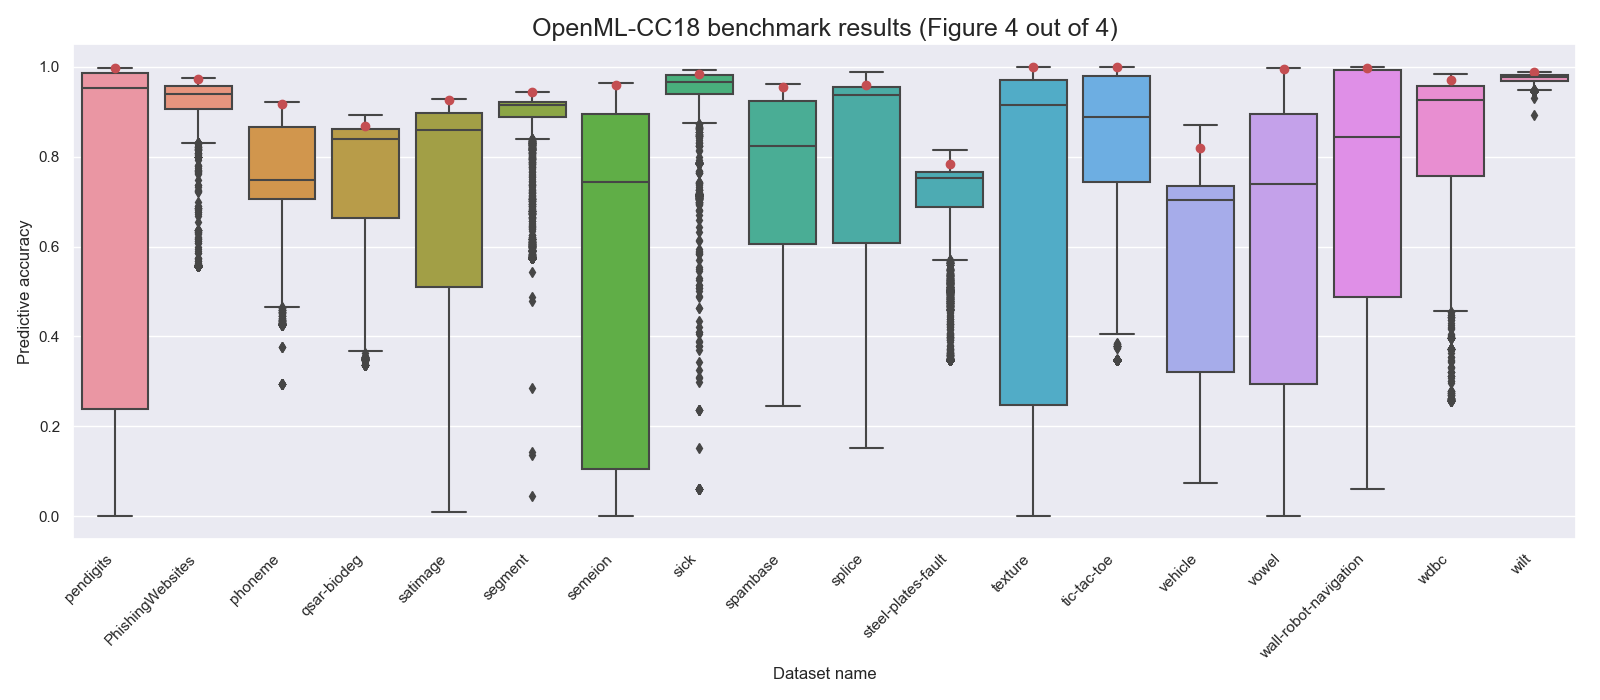
\includegraphics[width=\textwidth]{../img/openml-boxplot3.png}
    \caption[OpenML-CC18 benchmark result comparison (Figure 4 out of 4)]{
    OpenML-CC18 benchmark result comparison (Figure 4 out of 4).
    Boxplots visualize distributions of predictive accuracies of all
    runs uploaded to OpenML. Red circles mark our accuracy score on datasets.}
    \label{fig:OpenML:boxplot:3}
\end{sidewaysfigure}